\begin{itemize}


\item Processing: 
 
            \begin{figure}[h] 
            \centering
            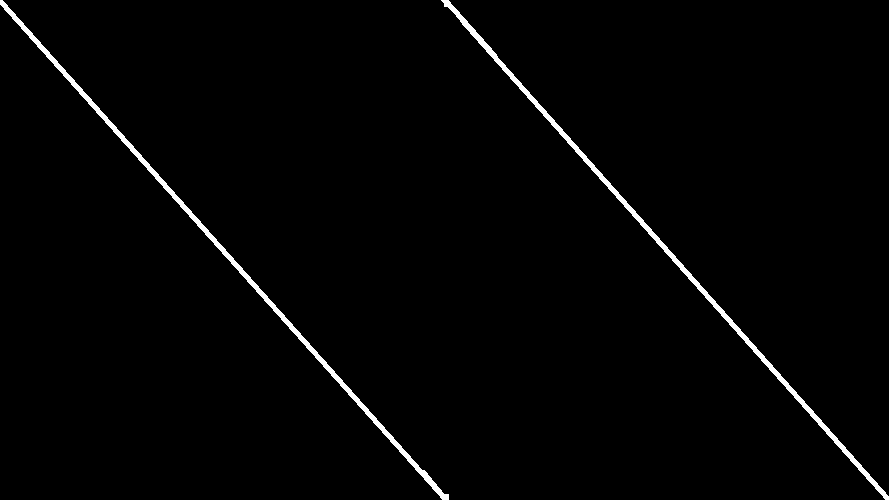
\includegraphics[width=2in]{Figures/testing/45Degrees.png}
            \caption{Test image with of 889 png by 500 png}
            \label{fig:processing_vertical_strips}
            \end{figure}   


    A test was made to check vertical strips produced in the program. The vertical strips function is one of the most important functions which enables the rest of the functions to work.
    Figure \ref{fig:processing_vertical_strips} was used with dimensions of 889 x 500 png. Processing.vertical\_strips() sections the image into equal sections by dividing the image width by an integer starting from 15. The function should only return the number 7. If it doesn't there is a problem with the code. 
    \item Connectivity:
    
    Connectivity.otsu() transforms grey-scale image like Figure \ref{fig:gradient_in} to a black and white image, Figure \ref{fig:Grad_Out}. By comparing the Numpy data array of the we can check the efficacy of the function.
    
    
    \noindent
        \begin{figure}
             \centering
             \begin{subfigure}[b]{0.3\textwidth}
                 \centering
                 
\includegraphics[width=\textwidth]{Figures/testing/Gradient.png}
                 \caption{Light to dark gradient used for testing thresholding calculation}
                 \label{fig:gradient_in}
             \end{subfigure}
             
             \begin{subfigure}[b]{0.3\textwidth}
                 \centering
                 
\includegraphics[width=\textwidth]{Figures/testing/Gradient_out.png}
                 \caption{Output image for test gradient}
                 \label{fig:Grad_Out}
             \end{subfigure}
            
            \caption{Input and Output Images for thresholding test}
            \label{fig:two gradients}
        \end{figure}
    
    \item Parameters:
        One of the main aims of the code was to find the Hydride Continuity factor of micrographs produced. Figure \ref{fig:test_image_hcc2} was the image chosen to check HCC value. By substituting the length of each hydride and total length of the strip in equation \ref{HCC_eqn} , equation \ref{test_hcc_eqn} is produced. This gives the expected return value of the HCC function when Figure \ref{fig:test_image_hcc2} is used.
        
        \begin{figure}[h] 
        \centering
        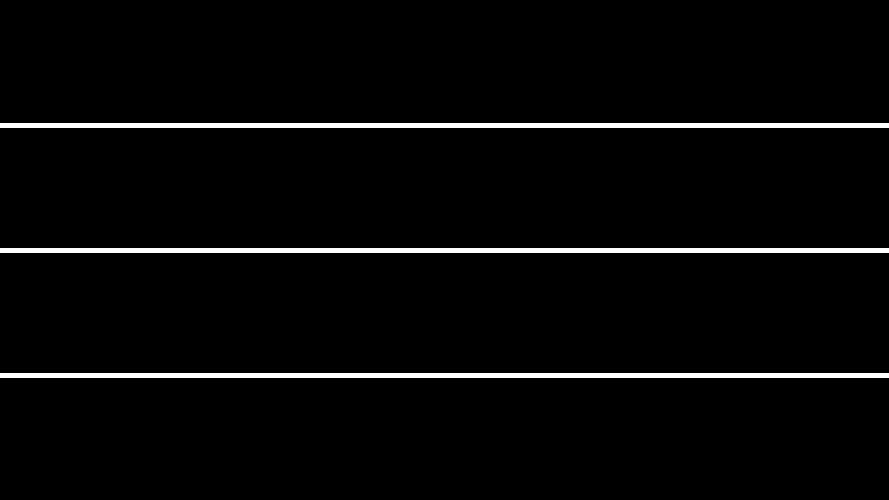
\includegraphics[width=2in]{Figures/testing/Full_Horizontal.png}
        \caption{Image to test HCC2 function}
        \label{fig:test_image_hcc2}
        \end{figure}
        
        \begin{equation} \label{test_hcc_eqn}
        \frac{3.68 + 3.68 + 3.68 }
                {133.86}
        = 0.0824742268
        \end{equation}
    
    \item For Gaussian thresholding two tests were created:
    
    \begin{enumerate}
        \item Tests whether after each treatment the input image and the output image had at least a 95\% similarity in terms of the image arrays. The test(s) was made to quickly determine whether a treatment (or its chosen parameters) had a large enough effect on the image to be considered useful.
        \item After the initial adaptive Gaussian thresholding, each pixel of the image was analyzed to determine whether it was white (value of 0) or black (value of 255). The test was made to confirm that the binarization had been successful and whether any possible subsequent treatment can rely on the fact the image is truly binary.
    
    \end{enumerate}
\end{itemize}